\documentclass[11pt,a4paper]{article}

% Packages
\usepackage[utf8]{inputenc}
\usepackage[T1]{fontenc}
\usepackage{lmodern}
\usepackage[margin=1in]{geometry}
\usepackage{graphicx}
\usepackage{amsmath,amssymb}
\usepackage{booktabs}
\usepackage{hyperref}
\usepackage{xcolor}
\usepackage{listings}
\usepackage{tikz}
\usepackage{float}
\usepackage{fancyhdr}
\usepackage{titlesec}
\usepackage{enumitem}

% Colors
\definecolor{qblue}{RGB}{41, 128, 185}
\definecolor{qdark}{RGB}{44, 62, 80}
\definecolor{qgreen}{RGB}{39, 174, 96}
\definecolor{qorange}{RGB}{230, 126, 34}
\definecolor{qred}{RGB}{192, 57, 43}
\definecolor{codebg}{RGB}{248, 248, 248}

% Hyperref setup
\hypersetup{
    colorlinks=true,
    linkcolor=qblue,
    filecolor=qblue,
    urlcolor=qblue,
    citecolor=qblue,
    pdftitle={Q-NarwhalKnight: Quantum-Enhanced VM and DEX},
    pdfauthor={Q-NarwhalKnight Development Team},
}

% Code listing style
\lstdefinestyle{rust}{
    backgroundcolor=\color{codebg},
    basicstyle=\ttfamily\small,
    breaklines=true,
    frame=single,
    rulecolor=\color{gray!30},
    keywordstyle=\color{qblue}\bfseries,
    commentstyle=\color{qgreen},
    stringstyle=\color{qorange},
    numbers=left,
    numberstyle=\tiny\color{gray},
    numbersep=5pt,
}

% Header/Footer
\pagestyle{fancy}
\fancyhf{}
\fancyhead[L]{\textcolor{gray}{\small Q-NarwhalKnight Whitepaper}}
\fancyhead[R]{\textcolor{gray}{\small v1.0.92-beta}}
\fancyfoot[C]{\thepage}
\renewcommand{\headrulewidth}{0.4pt}

% Title formatting
\titleformat{\section}{\Large\bfseries\color{qdark}}{\thesection}{1em}{}
\titleformat{\subsection}{\large\bfseries\color{qblue}}{\thesubsection}{1em}{}
\titleformat{\subsubsection}{\normalsize\bfseries\color{qdark}}{\thesubsubsection}{1em}{}

% Document
\begin{document}

% Title Page
\begin{titlepage}
    \centering
    \vspace*{2cm}

    {\Huge\bfseries\textcolor{qdark}{Q-NarwhalKnight}\par}
    \vspace{0.5cm}
    {\LARGE\textcolor{qblue}{Quantum-Enhanced Virtual Machine\\and Decentralized Exchange}\par}

    \vspace{1.5cm}
    {\Large\textbf{Technical Whitepaper v1.0}\par}

    \vspace{2cm}

    % Simple diagram using TikZ
    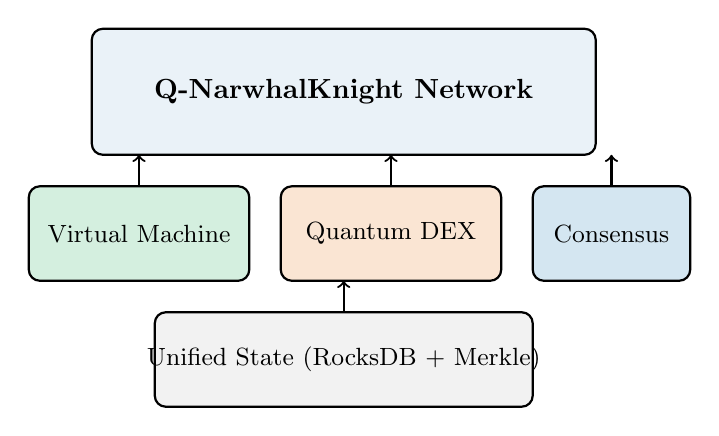
\begin{tikzpicture}[scale=0.8]
        \draw[thick, fill=qblue!10, rounded corners] (-4,-1) rectangle (4,1);
        \node at (0,0) {\textbf{Q-NarwhalKnight Network}};

        \draw[thick, fill=qgreen!20, rounded corners] (-5,-3) rectangle (-1.5,-1.5);
        \node at (-3.25,-2.25) {\small Virtual Machine};

        \draw[thick, fill=qorange!20, rounded corners] (-1,-3) rectangle (2.5,-1.5);
        \node at (0.75,-2.25) {\small Quantum DEX};

        \draw[thick, fill=qblue!20, rounded corners] (3,-3) rectangle (5.5,-1.5);
        \node at (4.25,-2.25) {\small Consensus};

        \draw[thick, fill=gray!10, rounded corners] (-3,-5) rectangle (3,-3.5);
        \node at (0,-4.25) {\small Unified State (RocksDB + Merkle)};

        \draw[->, thick] (-3.25,-1.5) -- (-3.25,-1);
        \draw[->, thick] (0.75,-1.5) -- (0.75,-1);
        \draw[->, thick] (4.25,-1.5) -- (4.25,-1);
        \draw[->, thick] (0,-3.5) -- (0,-3);
    \end{tikzpicture}

    \vfill

    {\large Q-NarwhalKnight Development Team\par}
    \vspace{0.5cm}
    {\large December 2025\par}

    \vspace{1cm}
    {\small\texttt{https://quillon.xyz}\par}
\end{titlepage}

% Abstract
\begin{abstract}
\noindent Q-NarwhalKnight introduces a novel blockchain architecture that combines a post-quantum secure virtual machine with a physics-inspired decentralized exchange. The system leverages quantum mechanical concepts---superposition, entanglement, and wave function collapse---as metaphors for advanced trading mechanics while implementing genuine post-quantum cryptographic primitives for future-proof security. This paper describes the technical architecture, execution model, pricing algorithms, and security mechanisms of the integrated VM-DEX platform.

\vspace{0.5cm}
\noindent\textbf{Keywords:} Blockchain, Virtual Machine, Decentralized Exchange, Post-Quantum Cryptography, AMM, DAG Consensus
\end{abstract}

\newpage
\tableofcontents
\newpage

%------------------------------------------------------------------------------
\section{Introduction}
%------------------------------------------------------------------------------

\subsection{Motivation}

Current blockchain virtual machines face three fundamental challenges:

\begin{enumerate}[leftmargin=*]
    \item \textbf{Quantum Vulnerability}: Existing cryptographic primitives (ECDSA, Ed25519) will be broken by sufficiently powerful quantum computers.
    \item \textbf{DEX Inefficiency}: Traditional AMMs suffer from impermanent loss, front-running, and inefficient price discovery.
    \item \textbf{Fragmented Architecture}: Smart contracts and DEX functionality typically exist as separate, loosely-coupled systems.
\end{enumerate}

Q-NarwhalKnight addresses these challenges through an integrated architecture where the virtual machine and decentralized exchange share state, security primitives, and consensus mechanisms.

\subsection{Key Innovations}

\begin{itemize}[leftmargin=*]
    \item \textbf{Post-Quantum Security}: Dilithium5 signatures and Kyber1024 key encapsulation
    \item \textbf{Physics-Inspired AMM}: Golden ratio optimization and uncertainty-based pricing
    \item \textbf{Unified State Model}: Contracts and DEX pools share atomic state transitions
    \item \textbf{DAG-Knight Consensus}: Zero-message-complexity Byzantine agreement
\end{itemize}

\subsection{Design Philosophy}

The system draws inspiration from quantum mechanics not as a marketing device, but as a rigorous mathematical framework for modeling uncertainty, correlation, and state transitions in financial systems. The golden ratio $\varphi = 1.618...$ and Euler's number $e = 2.718...$ provide natural optimization targets for trading parameters.

%------------------------------------------------------------------------------
\section{System Architecture}
%------------------------------------------------------------------------------

\subsection{High-Level Overview}

The Q-NarwhalKnight network consists of three primary components that interact through a shared state layer:

\begin{table}[H]
\centering
\begin{tabular}{lll}
\toprule
\textbf{Component} & \textbf{Responsibility} & \textbf{State Access} \\
\midrule
Virtual Machine & Contract execution, state transitions & Read/Write \\
Quantum DEX & Trading, liquidity, price discovery & Read/Write \\
DAG-Knight & Ordering, finality, Byzantine agreement & Read \\
\bottomrule
\end{tabular}
\caption{Component responsibilities and state access patterns}
\end{table}

\subsection{State Model}

All state is represented as a Merkle-Patricia trie with the following structure:

\begin{lstlisting}[style=rust]
pub struct VmState {
    contracts: HashMap<Address, Vec<u8>>,           // Contract bytecode
    storage: HashMap<Address, HashMap<Key, Value>>, // Contract storage
    balances: HashMap<Address, u64>,                // Native token balances
    nonces: HashMap<Address, u64>,                  // Replay protection
    state_root: [u8; 32],                           // Merkle root
    block_height: u64,                              // Current height
}
\end{lstlisting}

State transitions are \textbf{atomic}: either all changes from a transaction apply, or none do. This guarantees consistency across the VM and DEX components.

%------------------------------------------------------------------------------
\section{Virtual Machine Design}
%------------------------------------------------------------------------------

\subsection{Execution Model}

The Q-NarwhalKnight VM executes smart contracts in a sandboxed WebAssembly (WASM) environment with the following characteristics:

\begin{itemize}[leftmargin=*]
    \item \textbf{Deterministic Execution}: Identical inputs produce identical outputs across all nodes
    \item \textbf{Metered Computation}: Gas limits prevent infinite loops and resource exhaustion
    \item \textbf{Memory Safety}: WASM's linear memory model prevents buffer overflows
    \item \textbf{Isolation}: Contracts cannot access host system resources directly
\end{itemize}

\subsection{Contract Types}

The VM supports a rich taxonomy of contract types:

\subsubsection{Token Contracts}

\begin{table}[H]
\centering
\begin{tabular}{lll}
\toprule
\textbf{Type} & \textbf{Description} & \textbf{Use Case} \\
\midrule
SecureToken & ERC20-compatible fungible token & Standard tokens \\
AdvancedToken & Extended functionality (mint, burn, pause) & Platform tokens \\
RwaToken & Real World Asset representation & Tokenized assets \\
OrbusdStablecoin & Algorithmic stablecoin & Stable value storage \\
\bottomrule
\end{tabular}
\caption{Token contract types}
\end{table}

\subsubsection{DeFi Contracts}

\begin{table}[H]
\centering
\begin{tabular}{lll}
\toprule
\textbf{Type} & \textbf{Description} & \textbf{Use Case} \\
\midrule
LiquidityPool & AMM liquidity pool & DEX trading pairs \\
LendingPool & Collateralized lending & Borrowing/lending \\
YieldFarming & Liquidity mining rewards & Incentive programs \\
StakingContract & Token staking for rewards & Network security \\
CollateralVault & CDP for stablecoin minting & QUGUSD creation \\
\bottomrule
\end{tabular}
\caption{DeFi contract types}
\end{table}

\subsection{Gas Model}

Computation is metered using a gas system to prevent resource exhaustion:

\begin{table}[H]
\centering
\begin{tabular}{lr}
\toprule
\textbf{Operation} & \textbf{Gas Cost} \\
\midrule
Simple arithmetic & 3 \\
Storage read & 200 \\
Storage write (new) & 20,000 \\
Storage write (existing) & 5,000 \\
Contract call & 700 + subcall gas \\
Token transfer & 21,000 \\
Contract deployment & 32,000 + bytecode\_length $\times$ 200 \\
\bottomrule
\end{tabular}
\caption{Representative gas costs}
\end{table}

%------------------------------------------------------------------------------
\section{Quantum-Enhanced DEX}
%------------------------------------------------------------------------------

\subsection{Physics-Inspired Design}

The DEX incorporates quantum mechanical concepts as rigorous mathematical models for trading dynamics.

\subsubsection{Quantum States}

Trading orders exist in one of three states:

\begin{enumerate}[leftmargin=*]
    \item \textbf{Superposition}: Order pending, multiple outcomes possible
    \item \textbf{Collapsed}: Order executed, state determined
    \item \textbf{Entangled}: Order correlated with another (e.g., arbitrage pair)
\end{enumerate}

\subsubsection{Physical Constants}

The system uses fundamental constants for parameter tuning:

\begin{table}[H]
\centering
\begin{tabular}{llp{6cm}}
\toprule
\textbf{Constant} & \textbf{Value} & \textbf{Application} \\
\midrule
Golden Ratio ($\varphi$) & 1.618033988749895 & Slippage reduction, yield boost \\
Euler's Number ($e$) & 2.718281828459045 & Exponential bonding curves \\
Pi ($\pi$) & 3.141592653589793 & Wave function calculations \\
Uncertainty Factor & 0.1618 ($\varphi - 1$) & Price uncertainty bounds \\
\bottomrule
\end{tabular}
\caption{Physical constants and their applications}
\end{table}

\subsection{Liquidity Pool Structure}

Each liquidity pool maintains comprehensive state:

\begin{lstlisting}[style=rust]
pub struct QuantumLiquidityPool {
    pool_id: String,
    token_a_reserve: BigDecimal,
    token_b_reserve: BigDecimal,
    total_shares: BigDecimal,
    fee_rate: BigDecimal,                    // Default: 0.3%
    quantum_k_invariant: BigDecimal,         // x * y = k
    wave_function_state: QuantumState,
    entanglement_strength: f64,              // Correlation coefficient
    price_uncertainty: BigDecimal,           // Heisenberg-inspired bounds
}
\end{lstlisting}

\subsection{Order Types and Privacy Tiers}

\begin{table}[H]
\centering
\begin{tabular}{llp{7cm}}
\toprule
\textbf{Order Type} & \textbf{Description} & \textbf{Execution} \\
\midrule
Market & Execute immediately & Instant, slippage possible \\
Limit & Execute at specified price or better & Queued until conditions met \\
StopLoss & Trigger at price threshold & Converts to market order \\
\bottomrule
\end{tabular}
\caption{Order types}
\end{table}

\begin{table}[H]
\centering
\begin{tabular}{clp{7cm}}
\toprule
\textbf{Tier} & \textbf{Name} & \textbf{Features} \\
\midrule
0 & Basic & Standard on-chain transaction \\
1 & Enhanced & Tor routing, IP obfuscation \\
2 & Maximum & ZK proofs, multi-hop Tor, delayed execution \\
3 & Quantum & Post-quantum signatures, maximum anonymity \\
\bottomrule
\end{tabular}
\caption{Privacy tiers}
\end{table}

%------------------------------------------------------------------------------
\section{Automated Market Maker}
%------------------------------------------------------------------------------

\subsection{Constant Product Formula}

The core pricing mechanism uses the constant product invariant:

\begin{equation}
x \cdot y = k
\end{equation}

Where:
\begin{itemize}[leftmargin=*]
    \item $x$ = Reserve of token A
    \item $y$ = Reserve of token B
    \item $k$ = Invariant (constant after each trade)
\end{itemize}

\subsection{Quantum-Enhanced Pricing}

The base formula is enhanced with physics-inspired adjustments:

\subsubsection{Price with Uncertainty}

\begin{equation}
P_{effective} = P_{base} \times (1 \pm \epsilon)
\end{equation}

Where $\epsilon = 0.1618$ (the golden ratio minus one), creating natural price bands that reduce arbitrage opportunities.

\subsubsection{Golden Ratio Slippage Reduction}

Slippage is reduced by a factor of the inverse golden ratio:

\begin{equation}
\text{slippage}_{reduced} = \text{slippage}_{base} \times \frac{1}{\varphi} = \text{slippage}_{base} \times 0.618
\end{equation}

\subsubsection{Impermanent Loss Protection}

Liquidity providers receive 85\% protection against impermanent loss:

\begin{equation}
V_{protected} = V_{current} + 0.85 \times (V_{ideal} - V_{current})
\end{equation}

\subsection{Swap Execution}

For a swap of $\Delta x$ tokens of A for tokens of B:

\begin{align}
y_{new} &= \frac{k}{x + \Delta x} \\
\Delta y &= y - y_{new} \\
\Delta y_{after\_fee} &= \Delta y \times (1 - f)
\end{align}

Where $f = 0.003$ (0.3\% fee).

\textbf{Example}: Swap 1,000 USDC for QUG with reserves (100,000 USDC, 50,000 QUG):

\begin{align*}
k &= 100,000 \times 50,000 = 5 \times 10^9 \\
y_{new} &= \frac{5 \times 10^9}{100,000 + 1,000} = 49,504.95 \\
\Delta y &= 50,000 - 49,504.95 = 495.05 \text{ QUG} \\
\Delta y_{after\_fee} &= 495.05 \times 0.997 = 493.56 \text{ QUG}
\end{align*}

\subsection{Liquidity Provision}

\subsubsection{Adding Liquidity}

Initial provision uses the geometric mean:
\begin{equation}
\text{shares}_{minted} = \sqrt{\text{amount}_a \times \text{amount}_b}
\end{equation}

Subsequent provisions:
\begin{equation}
\text{shares}_{minted} = \min\left(\frac{\text{amount}_a}{\text{reserve}_a}, \frac{\text{amount}_b}{\text{reserve}_b}\right) \times \text{total\_shares}
\end{equation}

\subsubsection{Removing Liquidity}

\begin{align}
\text{amount}_a &= \frac{\text{shares}_{burned}}{\text{total\_shares}} \times \text{reserve}_a \\
\text{amount}_b &= \frac{\text{shares}_{burned}}{\text{total\_shares}} \times \text{reserve}_b
\end{align}

%------------------------------------------------------------------------------
\section{Collateral and Stablecoin System}
%------------------------------------------------------------------------------

\subsection{QUGUSD Stablecoin}

QUGUSD is a crypto-collateralized stablecoin pegged to 1 USD, backed by QUG tokens.

\subsection{Collateralization Parameters}

\begin{table}[H]
\centering
\begin{tabular}{llp{6cm}}
\toprule
\textbf{Parameter} & \textbf{Value} & \textbf{Purpose} \\
\midrule
Minimum Collateral Ratio & 150\% & Ensure over-collateralization \\
Warning Ratio & 120\% & Alert position holders \\
Liquidation Ratio & 110\% & Trigger liquidation \\
Liquidation Bonus & 5\% & Incentivize liquidators \\
\bottomrule
\end{tabular}
\caption{Collateralization parameters}
\end{table}

\subsection{Position Health Levels}

\begin{table}[H]
\centering
\begin{tabular}{llll}
\toprule
\textbf{Ratio} & \textbf{Status} & \textbf{Color} & \textbf{Action} \\
\midrule
$> 150\%$ & Healthy & \textcolor{qgreen}{Green} & Normal operation \\
$120\% - 150\%$ & Warning & \textcolor{qorange}{Yellow} & Add collateral advised \\
$110\% - 120\%$ & Danger & \textcolor{qorange}{Orange} & Imminent liquidation \\
$< 110\%$ & Liquidatable & \textcolor{qred}{Red} & Can be liquidated \\
\bottomrule
\end{tabular}
\caption{Position health levels}
\end{table}

\subsection{Collateral Operations}

\subsubsection{Minting QUGUSD}

To mint QUGUSD, users lock QUG as collateral:

\begin{equation}
\text{QUGUSD}_{max} = \frac{\text{QUG}_{locked} \times P_{QUG}}{1.5}
\end{equation}

\textbf{Example}: Lock 10,000 QUG at \$2.00/QUG:
\begin{align*}
\text{Collateral value} &= 10,000 \times \$2.00 = \$20,000 \\
\text{Max QUGUSD} &= \frac{\$20,000}{1.5} = 13,333 \text{ QUGUSD}
\end{align*}

\subsubsection{Liquidation}

When collateral ratio falls below 110\%, liquidators can repay the debt and receive the collateral plus a 5\% bonus:

\begin{equation}
\text{Collateral}_{liquidator} = \text{Debt}_{repaid} \times \frac{1.05}{P_{QUG}}
\end{equation}

%------------------------------------------------------------------------------
\section{Security Architecture}
%------------------------------------------------------------------------------

\subsection{Post-Quantum Cryptography}

The system implements NIST-standardized post-quantum algorithms:

\begin{table}[H]
\centering
\begin{tabular}{llll}
\toprule
\textbf{Algorithm} & \textbf{Type} & \textbf{Security Level} & \textbf{Usage} \\
\midrule
Dilithium5 & Signature & NIST Level 5 & Transaction signing \\
Kyber1024 & KEM & NIST Level 5 & Key exchange \\
SPHINCS+ & Signature & NIST Level 5 & Long-term keys \\
\bottomrule
\end{tabular}
\caption{Post-quantum cryptographic algorithms}
\end{table}

\subsection{Smart Contract Security}

\subsubsection{Reentrancy Guard}

The system implements OpenZeppelin-style reentrancy protection using RAII patterns:

\begin{lstlisting}[style=rust]
pub struct ReentrancyGuard {
    execution_state: Arc<Mutex<HashMap<[u8; 32], ExecutionState>>>,
}

impl ReentrancyGuard {
    pub fn enter(&self, contract: [u8; 32]) -> Result<Guard> {
        // Acquire lock, prevent reentrant calls
        // Guard automatically releases on drop (RAII)
    }
}
\end{lstlisting}

\subsubsection{Role-Based Access Control}

\begin{lstlisting}[style=rust]
// Standard roles
const DEFAULT_ADMIN_ROLE: [u8; 32] = [0u8; 32];
const MINTER_ROLE: [u8; 32] = keccak256("MINTER_ROLE");
const PAUSER_ROLE: [u8; 32] = keccak256("PAUSER_ROLE");
const UPGRADER_ROLE: [u8; 32] = keccak256("UPGRADER_ROLE");
\end{lstlisting}

\subsection{DEX Security}

\begin{table}[H]
\centering
\begin{tabular}{llr}
\toprule
\textbf{Protection} & \textbf{Mechanism} & \textbf{Default} \\
\midrule
Slippage & Max price impact check & 5\% \\
Front-running & Commit-reveal optional & N/A \\
Flash loans & Single-block reentrancy check & Enabled \\
Oracle manipulation & TWAP with outlier rejection & 5 samples \\
\bottomrule
\end{tabular}
\caption{DEX security mechanisms}
\end{table}

%------------------------------------------------------------------------------
\section{Performance Optimization}
%------------------------------------------------------------------------------

\subsection{Parallel Block Verification}

Block verification is parallelized using Rayon for significant speedup:

\begin{lstlisting}[style=rust]
// v1.0.92-beta: Optimized batch verification
pub async fn verify_block_batch(&self, blocks: &[QBlock]) -> Result<usize> {
    // OPTIMIZATION #1: Parallel hash computation outside lock
    let block_hashes: Vec<[u8; 32]> = blocks
        .par_iter()
        .map(|block| blake3::hash(&serialize(&block.header)))
        .collect();

    // OPTIMIZATION #2: Single lock for entire batch
    let mut state = self.state.lock().await;
    // Process all blocks with pre-computed hashes
}
\end{lstlisting}

\textbf{Performance Improvement}: 10-50x faster verification (5ms vs 50ms per 1000 blocks)

\subsection{Performance Characteristics}

\begin{table}[H]
\centering
\begin{tabular}{lrr}
\toprule
\textbf{Operation} & \textbf{Latency} & \textbf{Throughput} \\
\midrule
Block verification & 5 $\mu$s/block & 200,000 blocks/sec \\
State read & 10 $\mu$s & 100,000 reads/sec \\
State write & 50 $\mu$s & 20,000 writes/sec \\
Swap execution & 100 $\mu$s & 10,000 swaps/sec \\
Contract call & 1 ms & 1,000 calls/sec \\
\bottomrule
\end{tabular}
\caption{Performance characteristics}
\end{table}

%------------------------------------------------------------------------------
\section{Economic Model}
%------------------------------------------------------------------------------

\subsection{Token Distribution}

\textbf{QUG (Native Token)}:
\begin{itemize}[leftmargin=*]
    \item Total Supply: 21,000,000 QUG
    \item Mining Rewards: 50\% (10,500,000 QUG)
    \item Development: 20\% (4,200,000 QUG)
    \item Community: 30\% (6,300,000 QUG)
\end{itemize}

\subsection{Fee Structure}

\begin{table}[H]
\centering
\begin{tabular}{llp{5cm}}
\toprule
\textbf{Action} & \textbf{Fee} & \textbf{Recipient} \\
\midrule
Swap & 0.3\% & LPs (0.25\%) + Protocol (0.05\%) \\
Contract deployment & 1 QUG & Burned \\
Transaction & 0.001 QUG min & Validators \\
Liquidation & 5\% bonus & Liquidator \\
\bottomrule
\end{tabular}
\caption{Fee structure}
\end{table}

\subsection{Incentive Alignment}

\begin{itemize}[leftmargin=*]
    \item \textbf{Liquidity Providers}: Earn trading fees proportional to share
    \item \textbf{Validators}: Earn transaction fees and block rewards
    \item \textbf{Stakers}: Earn staking rewards from protocol revenue
    \item \textbf{Developers}: Grant program for ecosystem development
\end{itemize}

%------------------------------------------------------------------------------
\section{Conclusion}
%------------------------------------------------------------------------------

Q-NarwhalKnight represents a significant advancement in blockchain architecture by integrating:

\begin{enumerate}[leftmargin=*]
    \item \textbf{Post-Quantum Security}: Future-proof cryptography protecting against quantum attacks
    \item \textbf{Unified VM-DEX Architecture}: Shared state model eliminating fragmentation
    \item \textbf{Physics-Inspired Trading}: Golden ratio optimization and uncertainty-based pricing
    \item \textbf{High Performance}: Parallelized verification and batched database operations
\end{enumerate}

The system provides a complete DeFi platform capable of supporting tokens, liquidity pools, lending, stablecoins, and derivatives---all secured by quantum-resistant cryptography and consensus.

\subsection{Future Work}

\begin{itemize}[leftmargin=*]
    \item \textbf{ZK-Rollups}: Layer 2 scaling with zero-knowledge proofs
    \item \textbf{Cross-Chain Bridges}: Interoperability with Ethereum, Bitcoin
    \item \textbf{AI Integration}: On-chain machine learning inference
    \item \textbf{Governance}: Decentralized protocol governance
\end{itemize}

%------------------------------------------------------------------------------
\section*{References}
%------------------------------------------------------------------------------

\begin{enumerate}[leftmargin=*]
    \item Danezis, G., et al. ``Narwhal and Tusk: A DAG-based Mempool and Efficient BFT Consensus.'' \textit{EuroSys 2022}.
    \item NIST. ``Post-Quantum Cryptography Standardization.'' 2024.
    \item Adams, H., et al. ``Uniswap v2 Core.'' 2020.
    \item Buterin, V. ``Ethereum: A Next-Generation Smart Contract Platform.'' 2014.
\end{enumerate}

\vfill

\begin{center}
\rule{0.5\textwidth}{0.4pt}

\textbf{Document Version}: 1.0 \quad | \quad \textbf{Last Updated}: December 2025

\texttt{https://quillon.xyz}
\end{center}

\end{document}
